%\chapter{\leavevmode}
\chapter{\leavevmode Research Design}
% \chapter*{Proposed Research}
% \addcontentsline{toc}{chapter}{Proposed Research}
\label{chap:researchdesign}


% Research Objectives
% The goal of the research is to get an idea of what the potential "threat map" looks like.
% With the technical "specs" for the hardware and OS, can we manipulate device capabilities?
% What capabilities can we extend or add?

%% \section*{Research Objectives }
%% \addcontentsline{toc}{section}{Research Objectives}
% \section{Research Objectives }  \label{researchobjectives}

% The goal of this research is to understand the security and threat landscape of serial print device environments; the devices themselves as well as communication between the guest and host. Whether the hardware can support adding unintended functionality at the application and physical layers. And, with what we know about the USB standard and developing real time operating systems, can that functionality be used to create a dual purpose device (e.g., HID clone)?


% % \section*{Research Questions/Hypotheses}
% % \addcontentsline{toc}{section}{Research Questions/Hypotheses}
% \section{Research Questions}  \label{researchquestions}

% The research questions this study aims to answer are as follows:

% \begin{itemize}
%   \item \textbf{RQ1:} What is the baseline or minimum hardware these devices are running?
%   \item \textbf{RQ2:} What software is being used on these devices? OS, libraries...
%   \item \textbf{RQ3:} Can the software/firmware be modified? FreeRTOS/ReconOS/VXWorks.
%   \item \textbf{RQ4:} If so, how much can be modified in memory? Is manually reflashing possible?
%   \item \textbf{RQ5:} Assuming reflashing is possible, can the original OS keep original functions and be used as a HID clone or hub?
% \end{itemize}


% \section*{Methodology}
% \addcontentsline{toc}{section}{Methodology}
\section{Design Process}  \label{designprocess}

The design process is divided into two parts, information collection and exploitation. Beginning with teardown of the equipment, identification of components, and then analysis of the firmware, networking, and lastly, the USB communications between the host and device. Using the information gathered within the first stage, modifications will be made to the firmware installed on the serial printer. Each step of the process shown in Figure \ref{fig:designprocess_diagram}, is described as follows:

\begin{figure}[ht]
    \centering
    {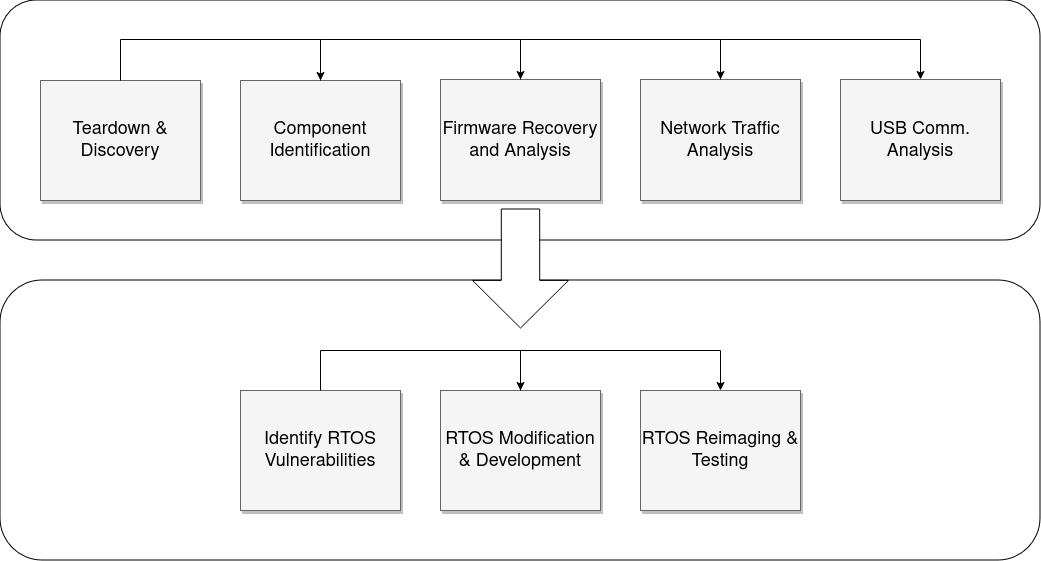
\includegraphics[width=148mm,scale=0.8]
    {Figures/Methodology_unlabeled.drawio.png}}
    \caption{Design process diagram}
    \label{fig:designprocess_diagram}
\end{figure}

% There are several parts to the methodology of the proposed research. First, technical information and datasheets must be collected for each of the identified devices. Then, device capabilities will be verified before beginning teardown and flash recovery. During the disassembly, each component will be documented and further technical information will be gathered from respective manufacturers. The format for presenting the collected data is described later in Section \ref{datacollectionprocess}.

\begin{itemize}
  \item \textbf{Teardown and Discovery:} The device is disassembled and documented at each step. Pictures are taken of each component, part numbers are identified, and technical datasheets are collected.
  \item \textbf{Component Identification:} Using information from the prior step, component function is identified and any information needed to interface with the component is documented.
  \item \textbf{Firmware Recovery and Analysis:} Using the technical datasheets, firmware is recovered and analyzed in a disassembler (e.g., Ghidra). Libraries used by the operating system and their opensource repositories are documented. Using the opensource information, potential vulnerabilities are identified within the firmware.
  \item \textbf{Network Traffic Analysis:} Any network traffic created during use is captured and analysed using software tools (e.g., WireShark). In conjuction with prior firmware analysis and identification of operating system libariries, communications are reviewed for potential vulnerabilities. This is a potential area for remote code execution (RCE) if the management software is poorly implemented.
  \item \textbf{USB Communication Analysis:} Communications between the host and device are captured for future development of human-interface-device (HID) cloning. The information is needed for accurately cloning identifiers assuming hosts restrict devices using vendor IDs. 
  \item \textbf{Identify RTOS Vulnerabilities:} Should analyses identify any exploitable vulnerabilities, further research is conducted to discover any public releases or proof of concepts (PoCs).
  \item \textbf{RTOS Modification and Development:} Opensource RTOS firmware is modified to allow HID cloning while maintaining original print functionality. The attack vector is crucial step towards proving viability of supply chain attacks using the print devices.
  \item \textbf{RTOS Reimaging and Testing:} Firmware is built and reimaged/reflashed onto the target device. Testing includes the verification of ESC/POS commands interpreter operation and HID attack vector. 
\end{itemize}

% \textbf{QUESTION: Should each of the bullet points have their own section explaining the process in detail?}

% Networking traffic will be analyzed according to NIST XYZ (?)...

% \textbf{PARAGRAPH OUTLINE:}
% \begin{itemize}
%   \item Find exact NIST guideline
%   \item Describe steps as described guideline
%   \item Tools used/needed
%   \item Why is network traffic analysis important?
%   \item How does this pertain to the end goal?
% \end{itemize}

% % What guidelines exactly? Is there a NIST guideline or research paper? Explain the steps and tools used.

% USB host-to-guest communications will be logged with Wireshark. This information will be needed for creation of HID cloning capabilities...

% \textbf{PARAGRAPH OUTLINE:}
% \begin{itemize}
%   \item Process for USB comm monitoring
%   \item How is this information used for HID cloning?
%   \item What information is needed exactly?
%   \item Tools used?
% \end{itemize}

% % ^ Explain how the USB communications will be analyzed. What will this information be used for exactly? How is it needed for understanding HID Cloning?

% The firmware will be recovered from flash and reviewed using Ghidra. The guidelines used for the assessment will follow .... XYZ .....

% \textbf{PARAGRAPH OUTLINE:}
% \begin{itemize}
%   \item Why are we reversing the firmware? What information are we looking for?
%   \item How are we reversing the firmware?
%   \item Tools used?
% \end{itemize}

% % Why are we reversing the firmware? What information are we looking for?
% % How are we reversing the firmware?

% Using the information gathered from the initial analysis of the print device, we will attempt to create a modified version of the operation system with HID cloning and existing functionality. This is to show that the device can either be compromised in the wild or prior as a part of a supply chain attack. HID cloning is then used as a method to demonstrate viable attacks against the host. 

% % Gather recent research within the last 5-10 years for manufacturer/device shares of the market
% % Gather technical sheets and specs for the most popular devices
% % Take note of the hardware specs for each device as well as firmware used
% % Create default/debug images of each popular devices' firmware - what is natively supported?
% % Is there room to add functionality without crippling original function


% \subsection{Research Approach} \label{researchapproach}

% For this research, the quantitative approach and case study research will be used \autocite{babbie2017basics,creswell2017research} to create a design artifact. The goal being to gather and examine, point-in-time, data from a serial printer device as a common sample representative of the affected population. By using quantitative survey research, it is possible to evaluate potential vulnerabilities for the attacks hypothesized, as well as, prototype a modified firmware image to use them against the host environment.

% \subsection{Cross-Sectional Survey} \label{casestudy}

% Using cross-sectional surveys \autocite{creswell2017research} has multiple benefits. It can be used to represent data as it is taken, rather than over a long period of time.  The study method also focuses on providing summaries that describe the patterns and context between collected data, and how it relates to the research questions.


\section{Data Collection Process} \label{datacollectionprocess}

The data collection process begins with gathering technical specifications from device manufacturers. Typically, these contain information about the capabilities of the intended device functions. For a printer, this could contain information ranging from hardware specifications (e.g., CPU, architecture, memory) to things like printed pages per minute. This information forms the baseline for the device survey. Afterwards, further specifications will be gathered for components as each device is disassembled and examined.

% Roughly, the types and format of gathered device specifications will appear as follows (e.g., SNBC BTP-S80 is used here):

% \begin{table}[ht]
%   \centering
%   \begin{tabular}{|p{4cm}|p{11cm}|}
%     \hline\rowcolor{gray!30}

%     \textbf{Specifications} &  \\
%     \hline

%     Max print speed & 120mm (Two-Color), 150mm (Grayscale), 250mm (Mono) \\
%     \hline

%     Printing method & Direct Thermal \\
%     \hline

%     Paper roll type & 9 x 7, 82.5 x 80 x 57.5mm \\
%     \hline

%     Bar code support & UPC-A, UPC-E, EAN8, EAN13, Code39, Code93, CODE128, CODABAR, ITF, PDF417, QR Code, Maxicode \\
%     \hline

%     Printer interpreter & ESC/POS \\
%     \hline

%     Interfaces & Serial+USB+Ethernet \\
%     &  USB+Parallel \\
%     &  USB+Serial \\
%     &  USB+Bluetooth \\
%     &  USB+WiFi \\
%     &  USB Only \\
%     \hline

%     Supported Host OS & 32-bit (Windows XP/2000/POSReady) \\
%     &  64bit (Windows XP/Server 2012) \\
%     &  32/64bit (Windows 10/8.1/8/7/Vista/Server 2008 or 2003) \\
%     &  Other (Linux/OPOS/BYJavaPOS Windows or Linux) \\
%     \hline

%     Development Kit & Android, iOS \\
%     \hline

%     Data Buffer & Receive Buffer RAM: 64KB \\
%      &  RAM Bitmap: 128KB \\
%      &  Flash Bitmap: 512KB \\
%     \hline

%     Power Supply & AC 100 $\sim$ 240V, 50/60 Hz Adapter \\
%     \hline

%     Power Usage & 2.0A / 60W \\
%     \hline

%     Safety and EMI & FCC/UL \\
%     \hline

%   \end{tabular}
%   \caption{Device specifications for SNBC BTP-S80}
%   \label{fig:device_specs}%
% \end{table}

% Following the previous example, the next step in the data collection process would be identifying the SoC. In the event that there is no beforehand knowledge, the SoC can be identified by comparing gathered datasheets during the components discovery. This is easily accomplished using an online service like FindChips \autocite{FindchipsElectronicPart}. The expected type and format for SoCs is described by Figure \ref{fig:soc_specs}.

The next step in the data collection process would be identifying the SoC. In the event that there is no beforehand knowledge, the SoC can be identified by comparing gathered datasheets during the components discovery. This is easily accomplished using an online service like FindChips \autocite{FindchipsElectronicPart}. The expected type and format for SoCs is described by Figure \ref{fig:soc_specs}.

The process for gathering flash/memory chip specifications is similar; identify serial number and manufacturer, then find the component datasheet. Gathering the pin layouts and format is useful for later stages, should manual flash recovery be needed. The expected format for memory chips can be seen at Figure \ref{fig:memory_specs}.

\begin{table}[H]
  \centering
  \begin{tabular}{|p{6cm}|p{9cm}|}
    \hline\rowcolor{gray!30}

    \textbf{Specifications} &  \\
    \hline

    Architecture & 32-bit ARM \\
    \hline

    Platform & ARM Cortex-M3 \\
    \hline

    Frequency & 80-MHz, 100DMIPS performance \\
    \hline

    Memory & 128KB single-cycle Flash memory \\
     & 64KB single-cycle SRAM \\
    \hline

    Firmware & Internal ROM loaded with StellarisWare \\
    \hline

    Advanced Comm. Interfaces & UART, SSI, I2C, I2S, CAN \\
    \hline

    Debug Interfaces & JTAG, SWD \\
    \hline

    Package format & 100-pin LQFP \\
    & 108-ball pin BGA \\
    \hline

  \end{tabular}
  \caption{SoC technical specs example using Stellaris LM3S2793 Microcontroller}
  \label{fig:soc_specs}%
\end{table}

The final report will contain each of these tables for the device and their identified core components. Operating system features and protections will be loosely summarized for the device,  and there is no set reporting format or requirements. The identified information will aid the final step of the process, creating a design artifact.

\begin{table}[H]
  \centering
  \begin{tabular}{|p{6cm}|p{9cm}|}
    \hline\rowcolor{gray!30}

    \textbf{Specifications} &  \\
    \hline

    Single power supply operation & 2.7 to 3.6V \\
    \hline

    Software Features & SPI Bus Compatible Serial Interface \\
    \hline

    Memory architecture & Uniform 64KB sectors \\
    & 256 byte page size \\
    \hline

    Programming & Page programming (up to 256 bytes) \\
    & Operations are page-by-page basis \\
    & Accelerated mode via 9V W\#/ACC pin \\
    & Quad page programming \\
    \hline

    Erase commands & Bulk erase function \\
     & Sector erase for 64KB sectors \\
     & Sub-sector erase for 4KB and 8KB sectors \\
    \hline

    Protections & W\#/ACC pin used with Status Register Bits to protect specified memory regions andconfigure parts as read-only \\
    & One time programmable area for permanent and secure identification \\
    \hline

    Package format & 16-pin SO \\
    & 8-contact WSON \\
    & 24-ball BGA, 5x5 pin config \\
    & 24 ball BGA, 6x6 pin config \\
    \hline

  \end{tabular}
  \caption{Memory specifications example using Infineon Technologies S25FL064P \autocite{S25FL064PSeriesFlash}}
  \label{fig:memory_specs}%
\end{table}

\section{Hardware Assessment} \label{hardwareassessment}

NIST SP 800-115 \autocite{NISTSP8001152020} provides general guidelines for performing information security testing and assessment, however, there is little information regarding hardware reverse engineering and firmware analysis. Their guidelines are aimed more towards single/multi-tasking operating systems like Windows or Unix-like, those where network logging and listener agents is feasible. For the targeted devices in this research proposal, a different approach is needed that evaluates hardware protections of the SoC and flash memory. 

Analysis of device components, once disassembled, requires using a hardware debugger tool with the correct interface. The majority of the targeted devices are expected to use joint test action group (JTAG) or single wire debugging (SWD). By referring to the manufacturer datasheet for a given SoC, it is possible to identify the pin layout for serial debugging access.

\begin{figure}[ht]%
  \centering
  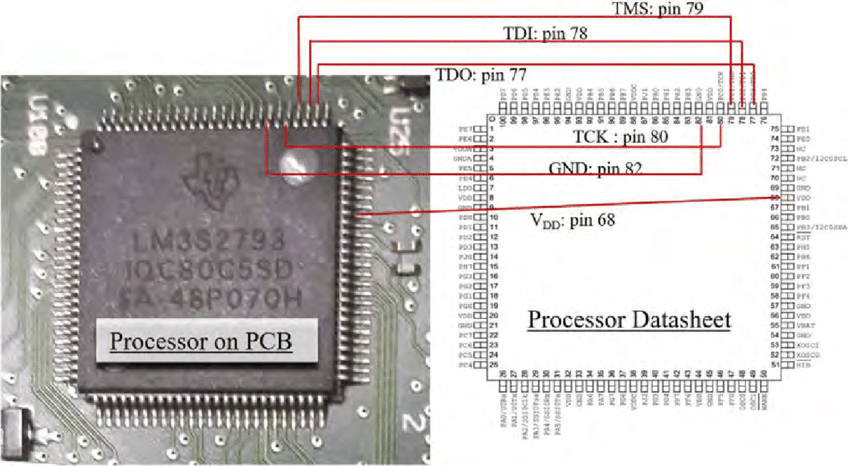
\includegraphics[keepaspectratio]{Figures/JTAGExample.png}
  \caption{JTAG pin out example for Texas Instruments LM3S2793}%
  \label{fig:jtag_pinout}%
\end{figure}

Figure \ref{fig:jtag_pinout} is an example showing what the physical SoC looks like on a PCB compared to the pin layout described in the datasheet. The dot in the top left of the SoC denotes the beginning of the pin layout. Counting in a counter-clockwise method indicates the pin number and the associated functions. For instance, to access the JTAG debug interface on the LM3S2793:

\begin{table}[H]
  \centering
  \begin{tabular}{|p{3cm}|p{3cm}|p{3cm}|p{3cm}|}

    

    \hline\rowcolor{gray!30}
    \textbf{Function} & \textbf{Pin \#} & \textbf{Function} & \textbf{Pin \#}  \\
    \hline

    TDO & 77 & TDI & 78 \\
    \hline

    TMS & 79 & TCK & 80 \\
    \hline

    GND & 82 & V\textsubscript{DD} & 68 \\
    \hline

  \end{tabular}
  \caption{example JTAG pin-out for the LM3S2793}
  % \caption{Memory specifications example using Infineon Technologies S25FL064P \autocite{S25FL064PSeriesFlash}}
  \label{table:example_jtag_pinout}%
\end{table}

Using this information, a device like the JTAGULATOR \autocite{JTAGulator2023} can be connected and enumerate or verify pin layouts as described. Ball joint SoCs require a different process and are much harder to debug if there is no visible header available on the board. Once an interface is connected, if debugger access is not disabled, the researcher can interact with the bootloader to further investigate enabled protections and recover flash storage.

If the JTAG is disabled, the researcher will then attempt to recover flash manually using a device like the Segger J-Link \autocite{SEGGERJLinkDebug}. The Segger has pre-defined and existing support for working with flash memory and flash breakpoints, whereas using OpenOCD with the JTAGULATOR would require time crafting custom configurations. Assuming there are no access protections to the flash memory, the researcher can begin performing firmware analysis to identify the operating system or potential vulnerabilities. Documenting the size and address range of memory regions is a key part of the process.

\section{Networking Traffic Analysis} \label{networkanalysis}

Work in progress.

\section{USB Communication Analysis} \label{usbcommanalysis}

Work in progress.

\section{RTOS Modification} \label{rtosmodification}

Work in progress.


